%!TEX root=../sts-template.tex
\section{Empirical analysis} % (fold)
\label{sec:empirical_analysis}

Using simulated data, we compare the estimation of the eigencomponents using the diagonalization of the covariance operator and the Gram matrix. The diagonalization of the covariance operator is performed using the methodology of \cite{happMultivariateFunctionalPrincipal2018a}. As this methodology is based on the expansion of each univariate feature into univariate principal components, we used univariate FPCA, if the curves are unidimensional, and the Functional Canonical Polyadic-Tensor Power Algorithm (FCP-TPA) for regularized tensor decomposition \citep{allenMultiwayFunctionalPrincipal2013a}, if the curves are two-dimensional. We choose the FCP-TPA as it is used by \cite{happMultivariateFunctionalPrincipal2018a} in their algorithm and implemented in their software \citep{happ-kurzObjectOrientedSoftwareFunctional2020}. Note that we could also use a two-dimensional basis expansion such as penalized tensor splines or discrete cosine transform, but we do not investigate these expansions here, as we do not want to prespecify a basis of functions.

The results of the simulation are compared using computation times (CT), the integrated squared error (ISE) risk function for the multivariate eigenfunctions, the log-absolute error ($\log-$AE) risk function for the eigenvalues and the mean integreated squared error (MISE) risk function for the reconstructed data. Let $\phi_k$ be the true eigenfunction and $\widehat{\phi}_k$ the estimated eigenfunction defined on $\TT{}$. We then define the ISE as, for $k = 1, \dots, K$,
\begin{equation}\label{eq:ise_eigenfunctions}
    \text{ISE}(\phi_k, \widehat{\phi}_k) = \normH{\phi_k - \widehat{\phi}_k}^2. %= \sum_{p = 1}^P \int_{\TT{p}} \{\phi^{(p)}_k(t_p) - \widehat{\phi}^{(p)}_k(t_p)\}^2 \dd t_p
\end{equation}
Let $\lambda = \{\lambda_1, \dots, \lambda_K\}$ be the set of true eigenvalues and $\widehat{\lambda} = \{\widehat{\lambda}_1, \dots, \widehat{\lambda}_K\}$ be the set of estimated eigenvalues. We then define the $\log-$AE as, for $k = 1, \dots, K$
\begin{equation}\label{eq:mse_eigenvalues}
    \log-\text{AE}(\lambda_k, \widehat{\lambda}_k) = \log(\lvert \lambda_k - \widehat{\lambda}_k\rvert).
\end{equation}
Let $\mathcal{X}$ be the set of true data and $\widehat{\mathcal{X}}$ be the set of reconstructed data. We define the MISE of the reconstructed data as
\begin{equation}\label{eq:mise_reconstructed_data}
    \text{MISE}(\mathcal{X}, \widehat{\mathcal{X}}) = \frac{1}{N}\sum_{n = 1}^N \normH{X_n - \widehat{X}_n}^2. %= \frac{1}{N}\sum_{n = 1}^N \sum_{p = 1}^P \int_{\TT{p}} \left\{\Xnp(t_p) - \hatXnp(t_p) \right\}^2 \dd t_p.
\end{equation}
Each integral is approximated by the trapezoidal rule with an equidistant grid. We let $\widehat{\phi}$, $\widehat{\lambda}$ and $\widehat{\mathcal{X}}$ be the estimators obtained using the Gram matrix and $\widetilde{\phi}$, $\widetilde{\lambda}$ and $\widetilde{\mathcal{X}}$ the estimators obtained using the covariance operator. For each simulation, we compute the ratios
\begin{equation}
    \frac{\text{ISE}(\phi_k, \widehat{\phi}_k)}{\text{ISE}(\phi_k, \widetilde{\phi}_k)}, \quad \frac{\log -\text{AE}(\lambda_k, \widehat{\lambda}_k)}{\log-\text{AE}(\lambda_k, \widetilde{\lambda}_k)},\quad k = 1, \dots, K,
\end{equation}
and
\begin{equation}
\frac{\text{MISE}(\mathcal{X}, \widehat{\mathcal{X}})}{\text{MISE}(\mathcal{X}, \widetilde{\mathcal{X}})},
\end{equation}
and compare them to $1$.

\subsection{Simulation experiments} % (fold)
\label{sub:simulation_experiments}

We consider two simulation scenarios. One consists of multivariate functional data with univariate features defined on one-dimensional domains and the other consists of univariate functional data defined on a two-dimensional domain.

\begin{scenario}
The simulation setting is based on the simulation in \cite{happMultivariateFunctionalPrincipal2018a}. The data-generating process is based on a truncated version of the Karhunen-Loève decomposition. First, we generate a large orthonormal basis $\{\psi_k\}_{1 \leq k \leq K}$ of $\sLp{\TT{}}$ on an interval $\TT{} = [0, T] \subset \RR$. We fix $T_1 = 0$ and $T_{P + 1} = T$ and we generate $P - 1$ cutting points $T_2, \dots, T_P$ uniformly in $\TT{}$ such that $0 = T_1 < \cdots < T_P < T_{P+1} = T$. Let $s_1, \dots, s_P \in \{-1, 1\}$ be coefficients that randomly flip the eigenfunctions with probability $0.5$. The univariate components of the eigenfunctions are then defined as, for $p = 1, \dots, P$, for $k = 1, \dots, K$,
\begin{equation}\label{eq:simulation_uni_component}
    \phi_k^{(p)}(t_p) = s_p \restr{\psi_k}{[T_p, T_{p + 1}]}\left(\frac{t_p - T_p}{T_{p + 1} - T_p}\right).
\end{equation}
The notation $\restr{\phi_k}{[T_p, T_{p + 1}]}$ is the restriction of the function $\phi_k$ to the set $[T_p, T_{p + 1}]$. The set of multivariate functions $\{\psi_k\}_{1 \leq k \leq K}$ is an orthonormal system in $\HH \coloneqq \sLp{\TT{1}} \times \dots \times \sLp{\TT{P}}$ with $\TT{p} = [0, 1]$. Each curve is then simulated using the truncated multivariate Karhunen-Loève expansion \eqref{eq:kl_multi_trunc}:
\begin{equation}
    X(\pointt) = \sum_{k = 1}^K \mathfrak{c}_k \phi_k(\pointt), \quad \pointt \in \TT{},
\end{equation}
where the scores $\mathfrak{c}_k$ are sampled as random normal variables with mean $0$ and variance $\lambda_k$. The eigenvalues $\lambda_k$ are defined with an exponential decrease, $\lambda_k = \exp(-(k + 1)/2)$. We simulate, for each replication of the simulation, $N = 25, 50, 75$ and $100$ observations. Similarly, each component is sampled on a regular grid of $M = 25, 50, 75$ and $100$ sampling points. We compare the methods for $P = 2, 10, 20$ and $50$ features and we set $K = 10$.
\end{scenario}

\begin{scenario}
The data generating process is again based on a truncated version of the Karhunen-Loève decomposition. First, we generate an orthonormal basis $\{\phi_k\}_{1 \leq k \leq K}$ of $\sLp{\TT{}}$ on an interval $\TT{} = [0, 1] \times [0, 1]$ as the tensor product of the first Fourier basis functions:
\begin{equation}
    \phi_k(s, t) = \psi_l(s) \otimes \psi_m(t), \quad s, t \in [0, 1],\ k = 1, \dots, K,
\end{equation}
where $\psi_l$ and $\psi_m$ are elements of the Fourier basis.
Each curve is then simulated using the truncated multivariate Karhunen-Loève expansion \eqref{eq:kl_multi_trunc}:
\begin{equation}
    X(s, t) = \sum_{k = 1}^K \mathfrak{c}_k \phi_k(s, t), \quad s, t \in [0, 1],
\end{equation}
where the scores $\mathfrak{c}_k$ are defined as for the Scenario~1. We simulate, for each replication of the simulations, $N = 25, 50, 75$ and $100$ observations. Similarly, each component is sampled on a regular grid of $M = 25 \times 25, 50 \times 50, 75 \times 75$ and $100 \times 100$ sampling points. We set $K = 10$.
\end{scenario}

% subsection simulation_experiments (end)

\subsection{Simulation results} % (fold)
\label{sub:simulation_results}

We compared MFPCA using the diagonalization of the covariance operator and using the diagonalization of the Gram matrix in terms of their CT, estimation of eigenvalues, estimation of eigenfunctions, and reconstruction of curves. We fix the number of retained components to be $5$ for each simulation of both scenarios. Each experiment is repeated $500$ times. The results are presented below.

% Computation time ----------
\begin{results}[Computational time.]
To compare the CT of the diagonalization of the covariance operator and the diagonalization of the Gram matrix, we measured the time it took for each method to complete the MFPCA for each simulated dataset.
Figure~\ref{fig:computation_time_mfd_1d} shows the kernel density estimates of the ratio of CT for each method across all sample sizes, number of sampling points and number of features. For Scenario 1, we found that the diagonalization of the covariance has a shorter CT compared to the diagonalization of the Gram matrix for most combinations of sample sizes, number of functions and number of sampling points. It is faster to use the Gram matrix if the number of observations is low compared to the number of sampling points.
%Note that the number of features $P$ does not change the ratio of CT between the methods.
\begin{figure*}
     \centering
    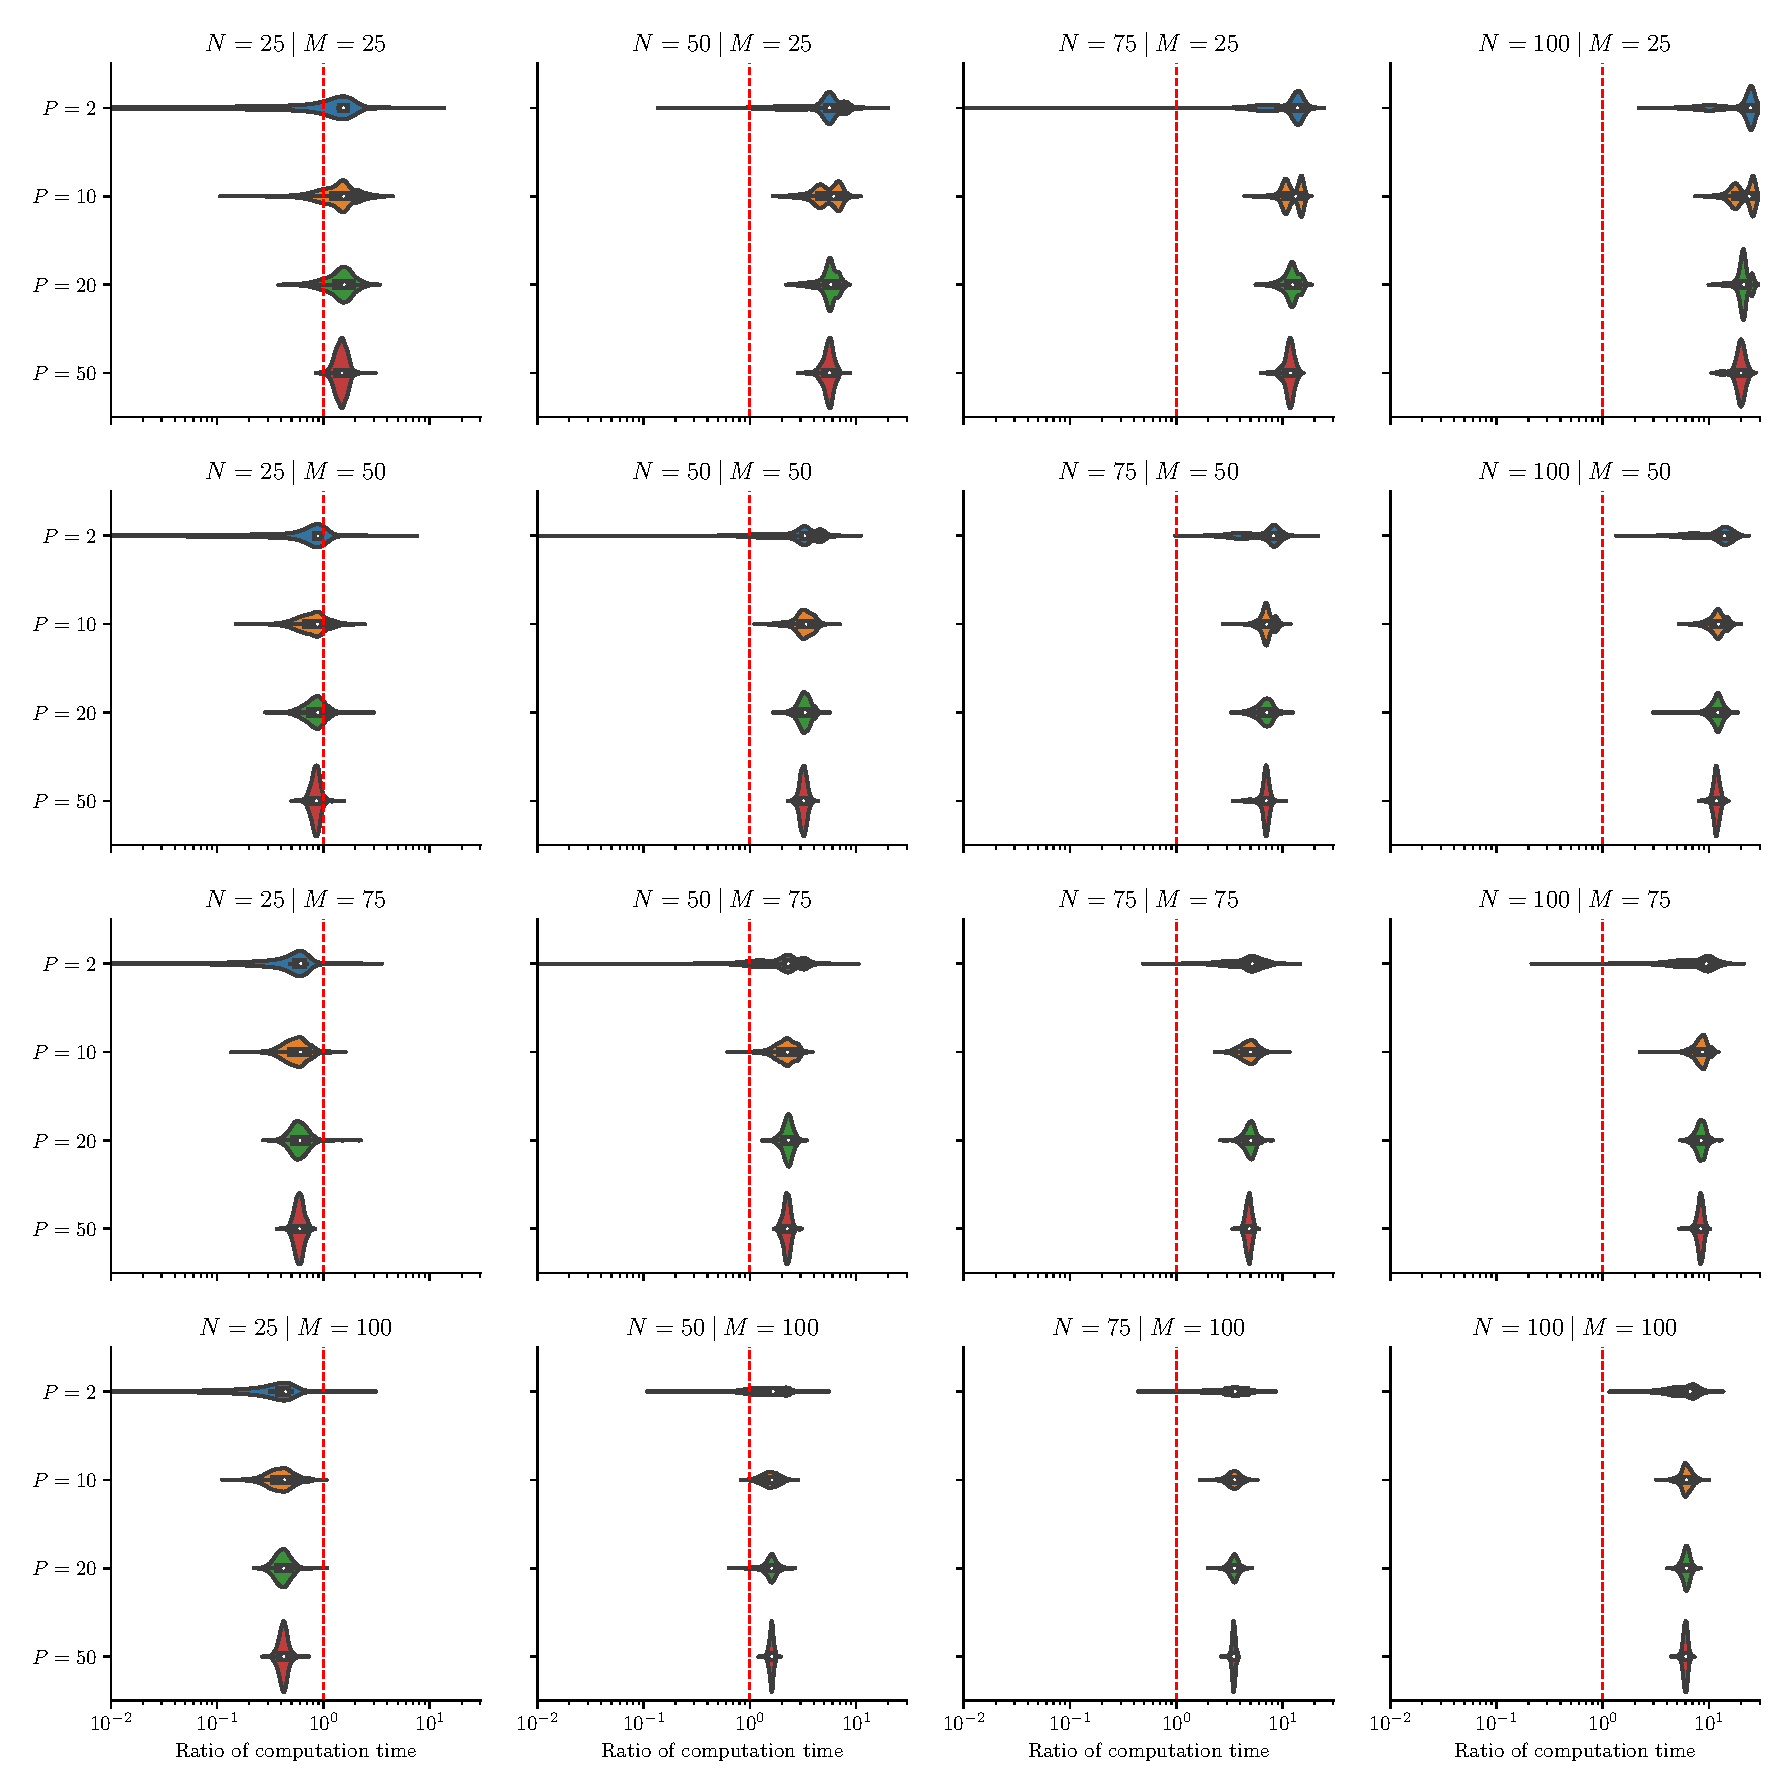
\includegraphics[width=0.95\textwidth]{figures/scenario_1/computation_time.eps}
    \caption{Ratio of computation time for Scenario 1 between the Gram matrix method and the covariance operator method. Each univariate component is defined on a one-dimensional domain. $N$ is the number of observations, $M$ is the number of sampling points per curve and $P$ is the number of features.}
    \label{fig:computation_time_mfd_1d}
\end{figure*}
Figure~\ref{fig:computation_time_mfd_2d} shows the kernel density estimates of the ratio of CT for each method across all sample sizes and number of sampling points. For Scenario 2, we found that the diagonalization of the Gram matrix has a shorter CT compared to the diagonalization of the covariance operator across all sample sizes and number of sampling points.
\begin{figure*}
     \centering
    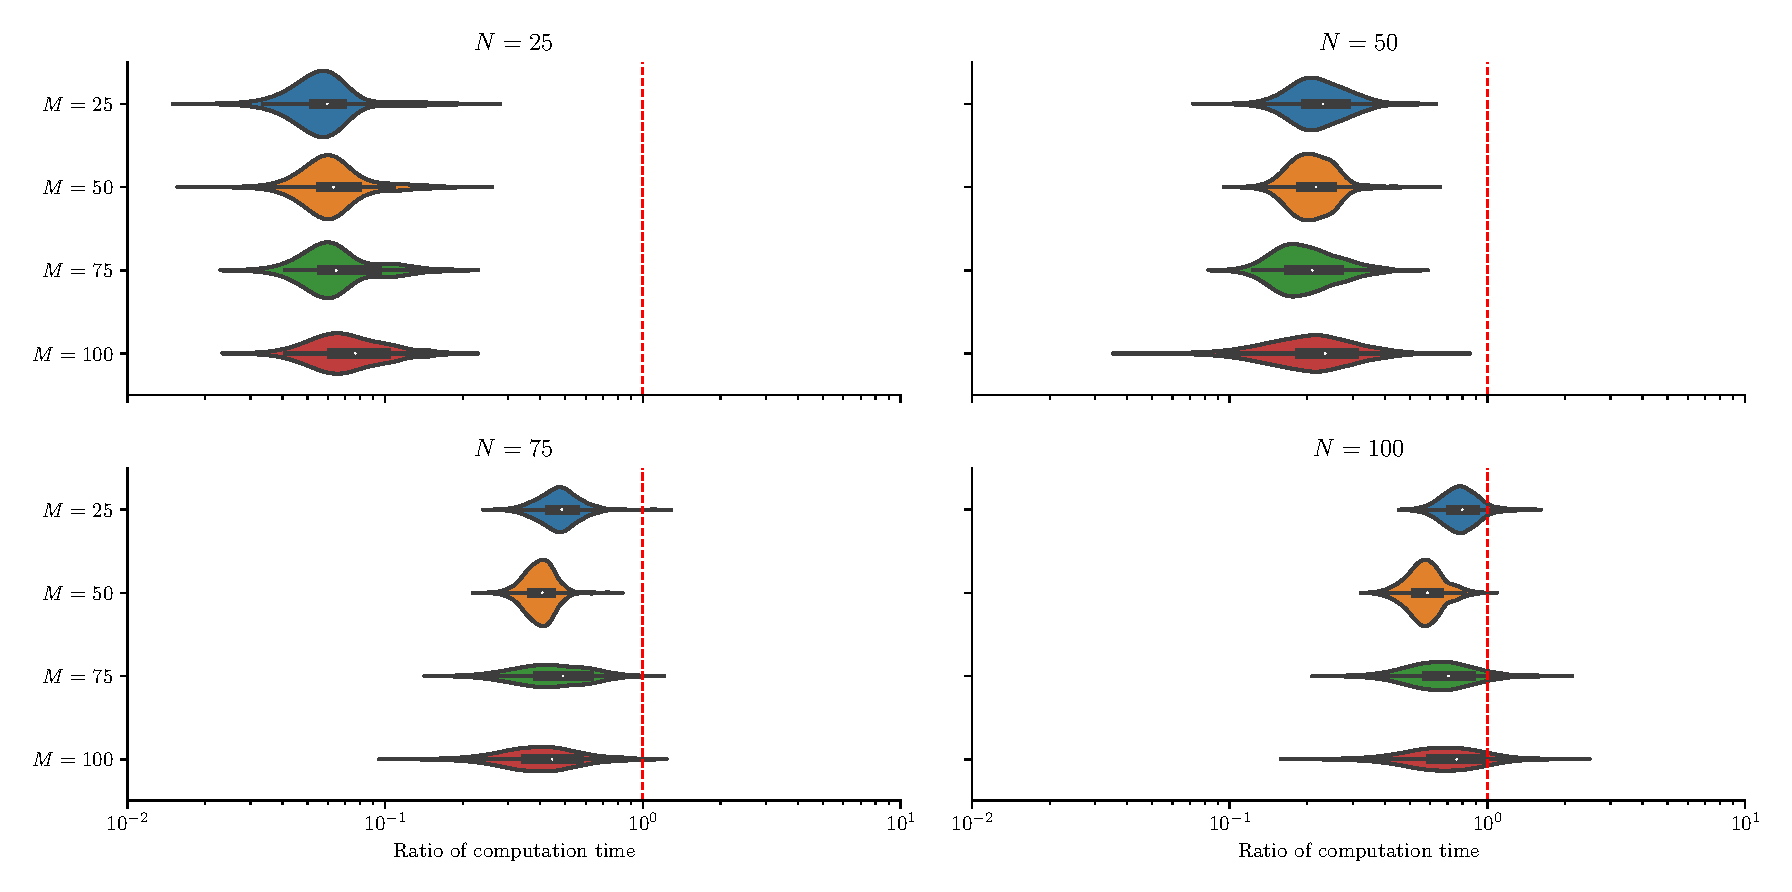
\includegraphics[width=0.95\textwidth]{figures/scenario_2/computation_time.eps}
    \caption{Ratio of computation time for Scenario 2 between the Gram matrix method and the covariance operator method. $N$ is the number of observations and $M \times M$ is the number of sampling points per images.}
    \label{fig:computation_time_mfd_2d}
\end{figure*}
The shorter CT of the diagonalization of the Gram matrix for  Scenario 2 makes it a more efficient option for analyzing two and higher-dimensional functional datasets. It is however worth noting that the CT can still vary depending on the specific implementation of each method, the computational resources available, and the complexity of the dataset (number of observations, number of sampling points, etc.).
\end{results}

% Eigenvalues estimation ----------
\begin{results}[Eigenvalues estimation.]
To compare the estimation of the eigenvalues between the diagonalization of the covariance operator and the diagonalization of the Gram matrix, we calculated the ratio of the $\log-\text{AE}$ \eqref{eq:mse_eigenvalues} between the estimated eigenvalues and the true eigenvalues for each simulated dataset and for the first five eigenvalues.
Figure~\ref{fig:logAE_mfd_1d} shows the boxplots of the $\log-\text{AE}$ for each method across all sample sizes, number of sampling points and number of features for Scenario 1. We found that the two methods behave similarly for all considered settings.
\begin{figure*}
    \centering
    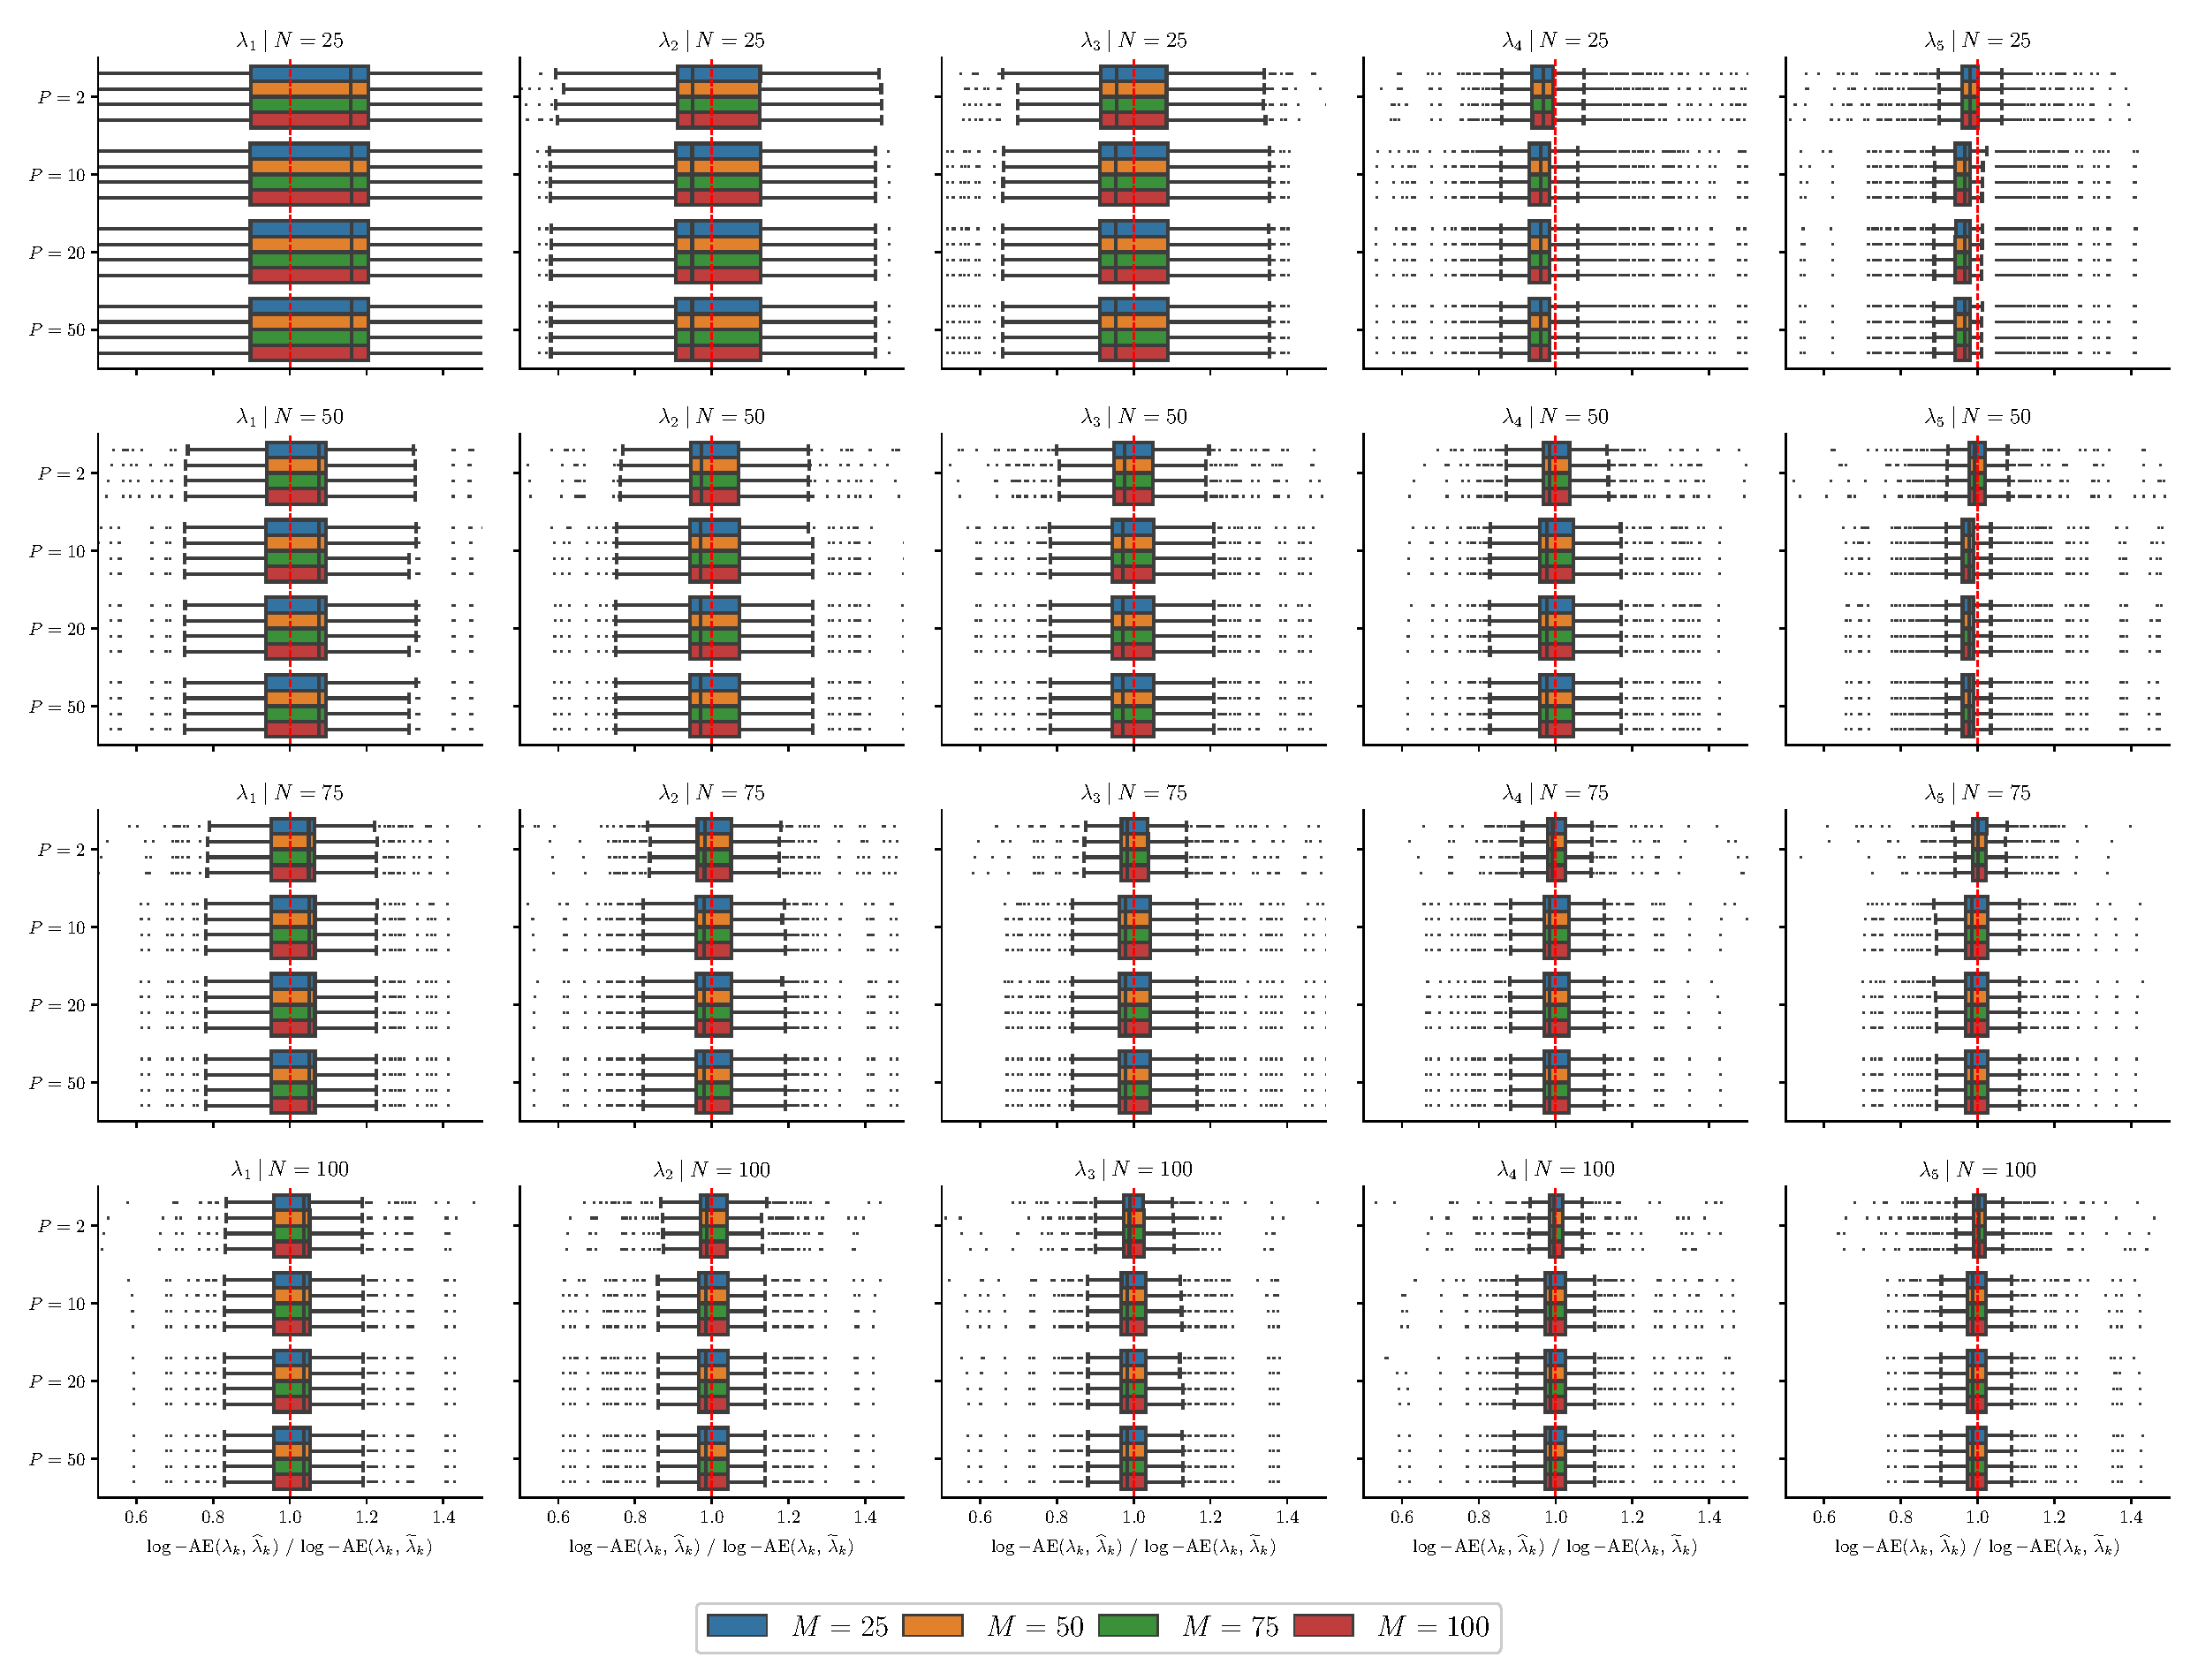
\includegraphics[width=0.95\textwidth]{figures/scenario_1/logAE.eps}
    \caption{Ratio of $\log-$AE for Scenario 1 between the Gram matrix method and the covariance operator method. Each univariate component is defined on a one-dimensional domain. $N$ is the number of observations, $M$ is the number of sampling points per curve and $P$ is the number of features.}
    \label{fig:logAE_mfd_1d}
\end{figure*}
Figure~\ref{fig:logAE_mfd_2d} shows the boxplots of the $\log-\text{AE}$ for each method across all sample sizes and number of sampling points for Scenario 2. We found that the FCP-TPA gives slighty better estimation of the eigenvalues.
\begin{figure*}
     \centering
    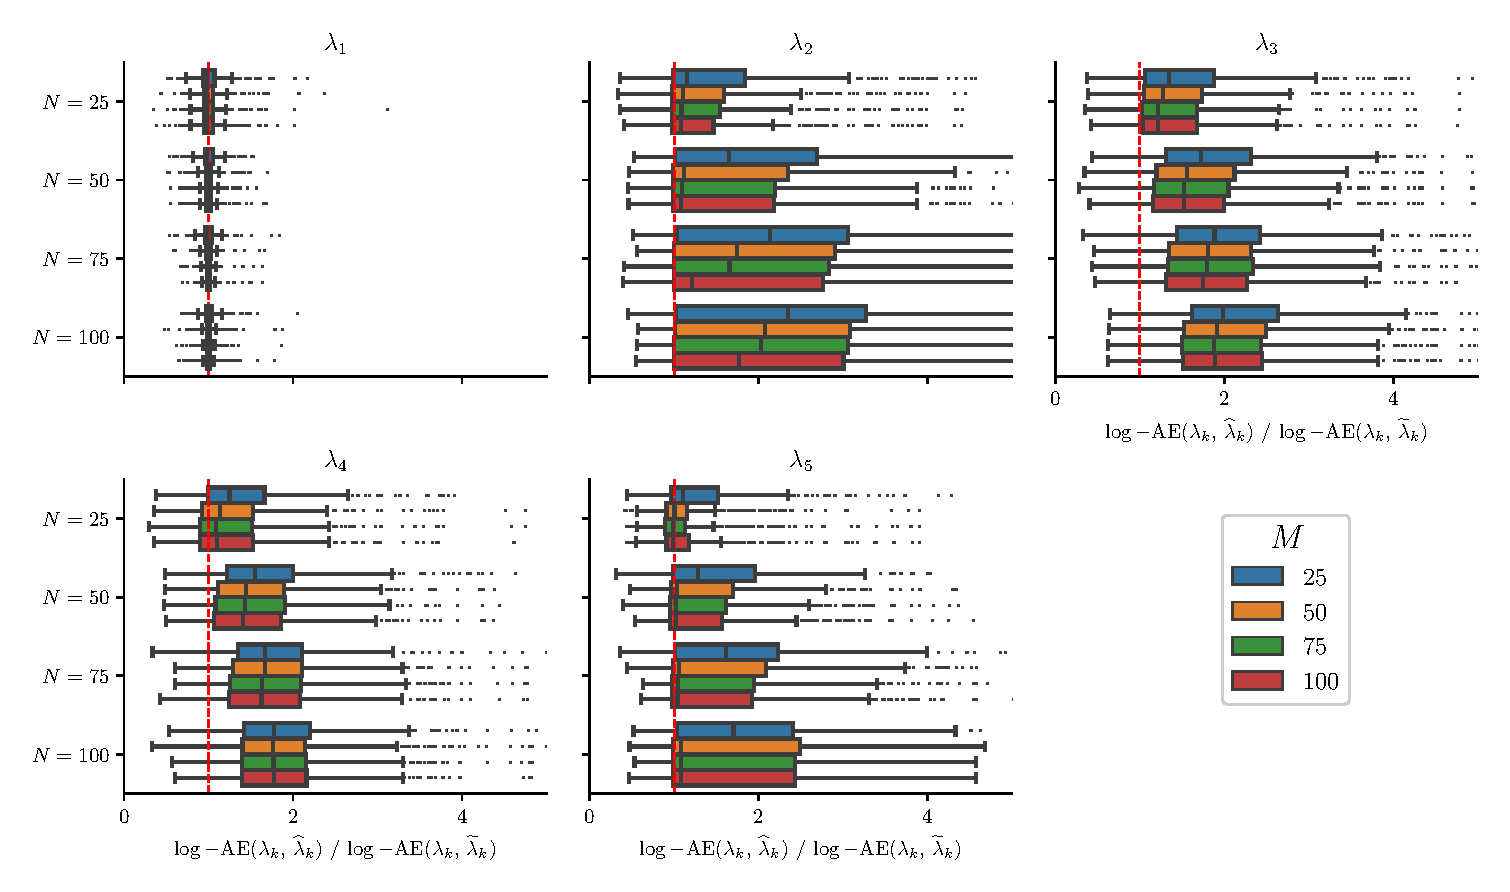
\includegraphics[width=0.95\textwidth]{figures/scenario_2/logAE.eps}
    \caption{Ratio of $\log-$AE for Scenario 2 between the Gram matrix method and the covariance operator method. $N$ is the number of observations and $M \times M$ is the number of sampling points per images.}
    \label{fig:logAE_mfd_2d}
\end{figure*}
\end{results}

% Eigenfunctions estimation ----------
\begin{results}[Eigenfunctions estimation.]
To compare the estimation of the eigenfunctions between the diagonalization of the covariance operator and the diagonalization of the Gram matrix, we calculated the ratio of the ISE \eqref{eq:ise_eigenfunctions} between the estimated eigenfunctions and the true eigenfunctions for each simulated dataset and for the first five eigenfunctions.
Figure~\ref{fig:ise_mfd_1d} shows the boxplots of the ISE for each method across all sample sizes, number of sampling points and number of features for Scenario 1. We found that the two methods behave similarly for all considered settings. For $P = 10, 20$ and $50$, the results are identical.
\begin{figure*}
     \centering
    \includegraphics[width=0.95\textwidth]{figures/scenario_1/ise.eps}
    \caption{Ratio of ISE for Scenario 1 between the Gram matrix method and the covariance operator method. Each univariate component is defined on a one-dimensional domain. $N$ is the number of observations, $M$ is the number of sampling points per curve and $P$ is the number of features.}
    \label{fig:ise_mfd_1d}
\end{figure*}
Figure~\ref{fig:ise_mfd_2d} shows the boxplots of the ISE for each method across all sample sizes and number of sampling points for Scenario 2. We found that the decomposition of the Gram matrix gives better estimation of the eigenfunctions compared to the FCP-TPA, especially when the number of observations increases.
\begin{figure*}
     \centering
    \includegraphics[width=0.95\textwidth]{figures/scenario_2/ise.eps}
    \caption{Ratio of ISE for Scenario 2 between the Gram matrix method and the covariance operator method. $N$ is the number of observations and $M \times M$ is the number of sampling points per images.}
    \label{fig:ise_mfd_2d}
\end{figure*}
\end{results}

% Curves reconstruction ----------
\begin{results}[Curves reconstruction.]
To compare the quality of the reconstruction of the curves between the diagonalization of the covariance operator and the diagaonlisation of the Gram matrix, we calculated the ratio of the MISE \eqref{eq:mise_reconstructed_data} between the reconstruction of the curves and the true curves for each simulated dataset.
Figure~\ref{fig:mise_mfd_1d} shows the boxplots of the ISE for each method across all sample sizes, number of sampling points and number of features for Scenario 1. We found that the diagonalization of the Gram matrix gives slightly better results for all considered settings.
\begin{figure*}
     \centering
     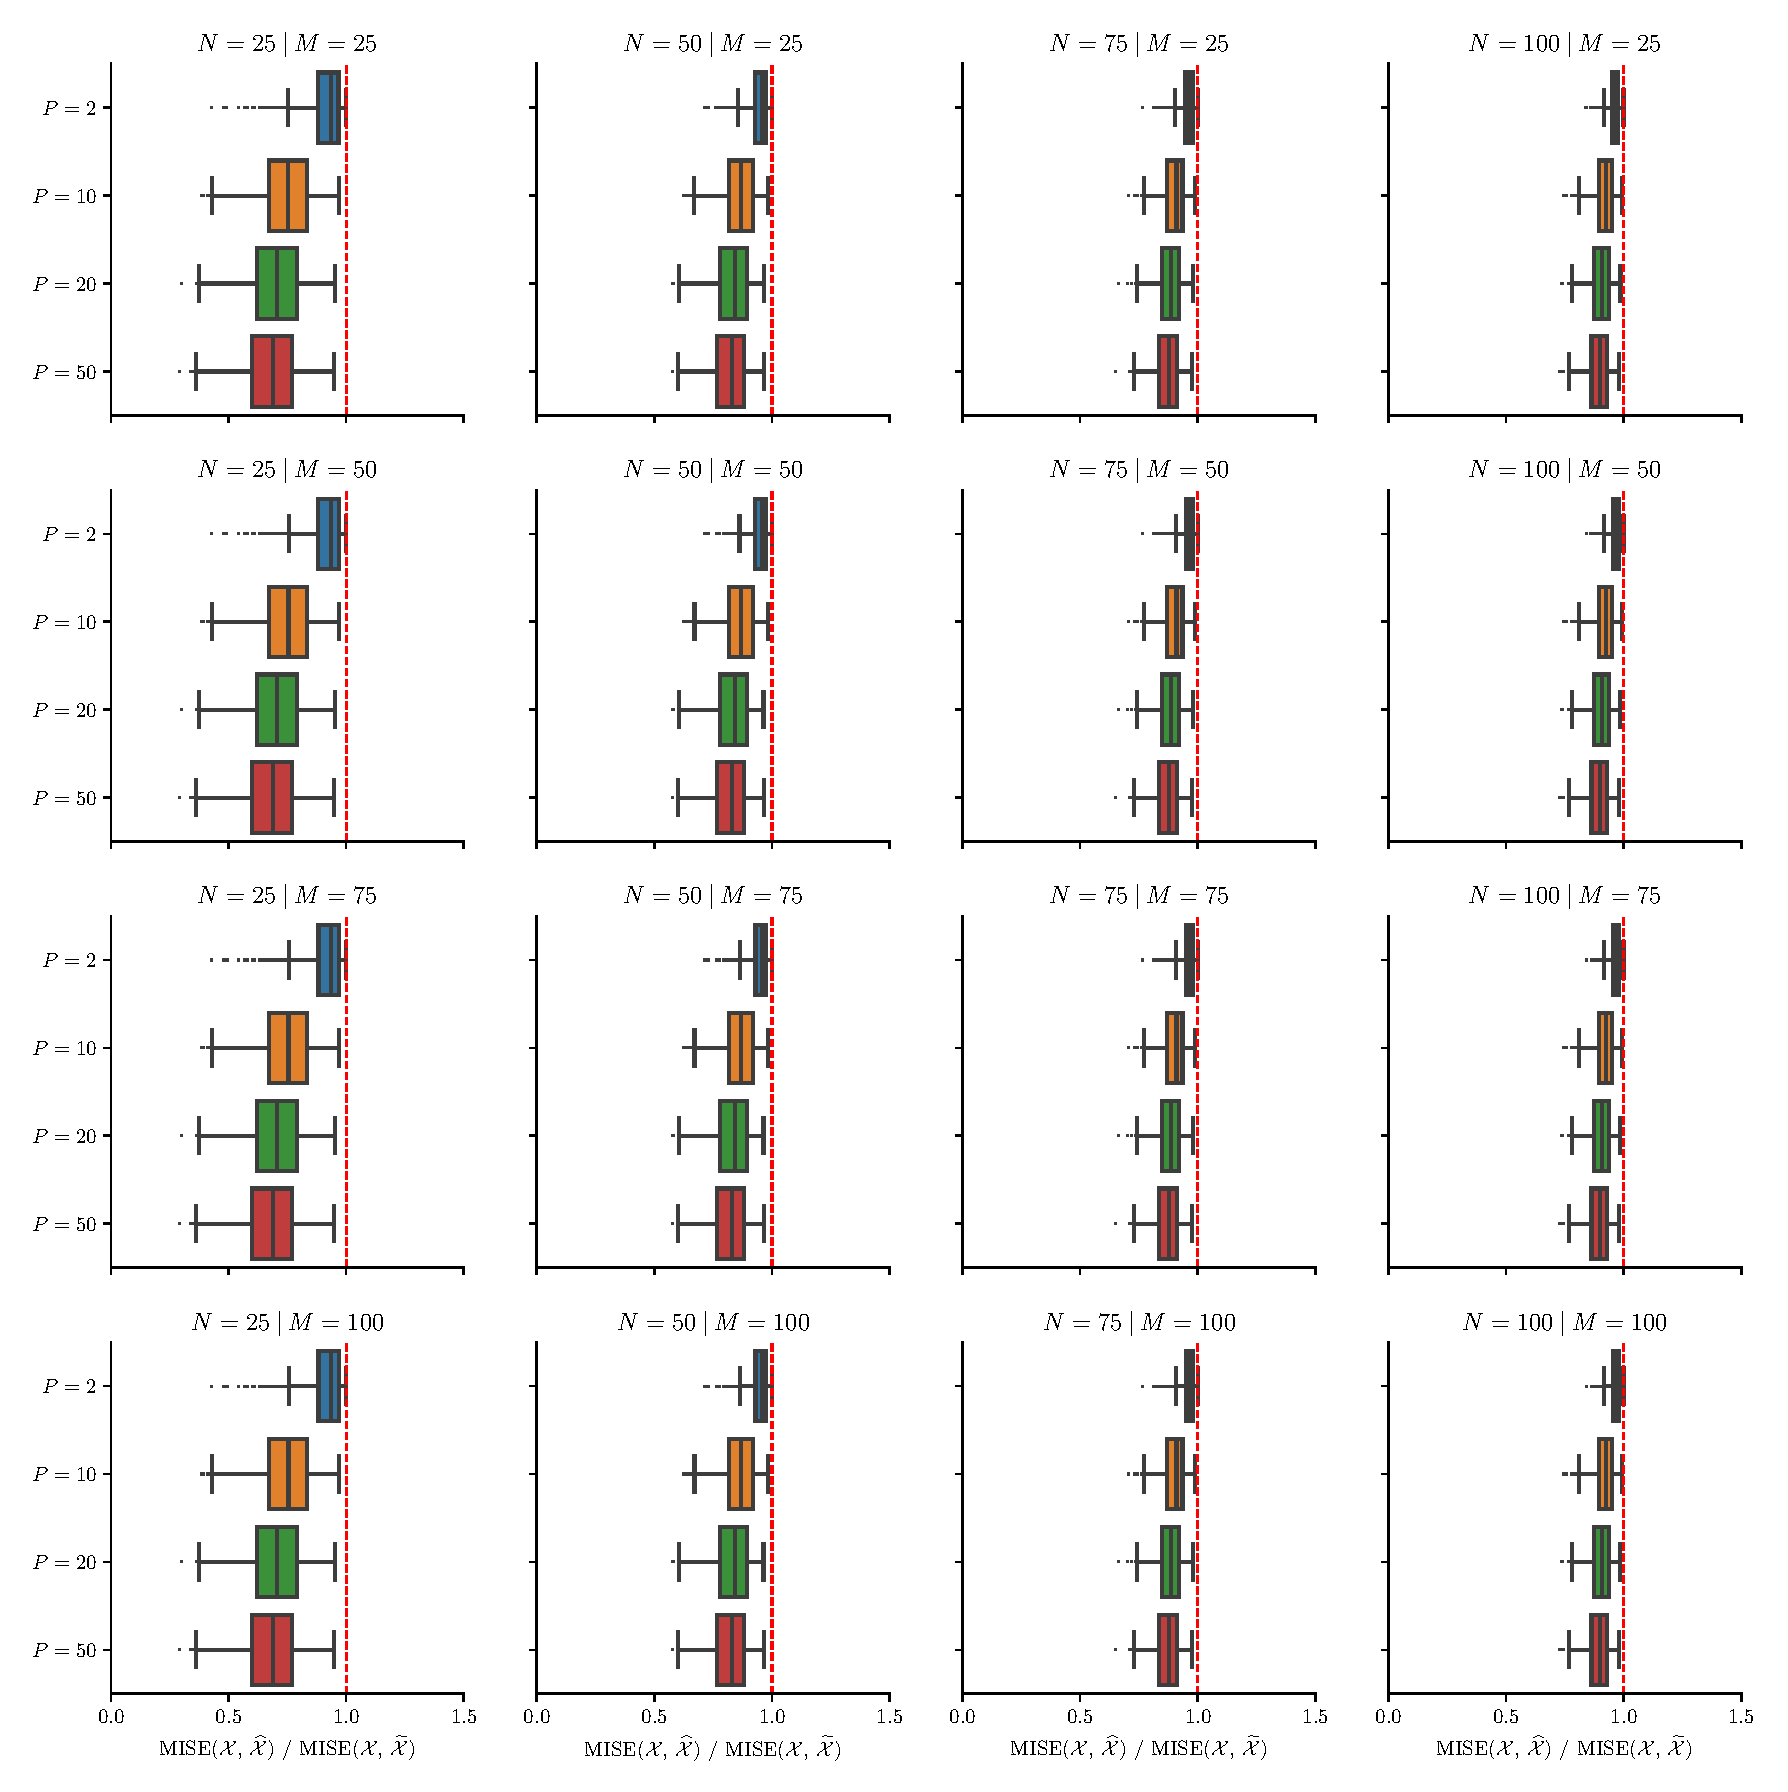
\includegraphics[width=0.95\textwidth]{figures/scenario_1/mise.eps}
    \caption{Ratio of MISE for Scenario 1 between the Gram matrix method and the covariance operator method. Each univariate component is defined on a one-dimensional domain. $N$ is the number of observations, $M$ is the number of sampling points per curve and $P$ is the number of features.}
    \label{fig:mise_mfd_1d}
\end{figure*}
Figure~\ref{fig:mise_mfd_2d} shows the boxplots of the ISE for each method across all sample sizes and number of sampling points for Scenario 2. Similarly to Scenario 1, we found that the decomposition of the Gram matrix gives better estimation of the true curves compared to the FCP-TPA, especially when the number of observations increases.
\begin{figure*}
     \centering
     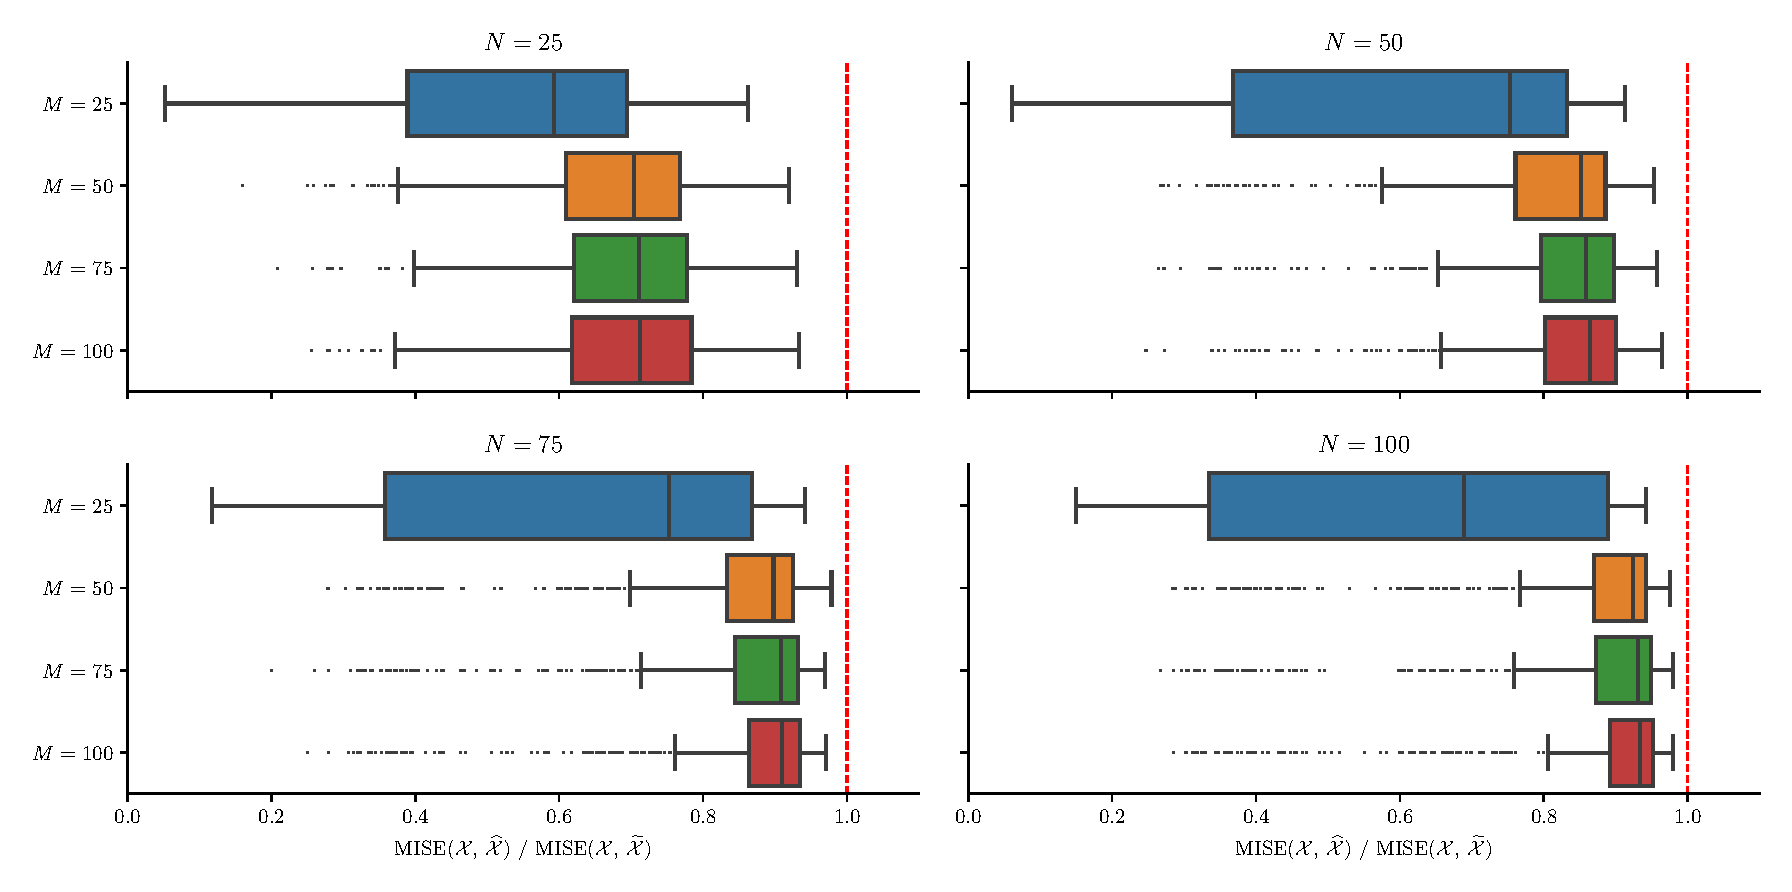
\includegraphics[width=0.95\textwidth]{figures/scenario_2/mise.eps}
    \caption{Ratio of MISE for Scenario 2 between the Gram matrix method and the covariance operator method. $N$ is the number of observations and $M \times M$ is the number of sampling points per images.}
    \label{fig:mise_mfd_2d}
\end{figure*}
\end{results}


% subsection simulation_results (end)

% \subsection{Percentage of variance explained} % (fold)
% \label{sub:percentage_of_variance_explained_simulation}

% \textcolor{red}{We argue that the percentage of variance explained in \cite{happMultivariateFunctionalPrincipal2018a} is sub-optimal as they consider the variance explained by each of the components separately and not the percentage explained overall. Using the inner product matrix however gives the correct number of eigenfunctions for a given amount of variance explained.
% We also consider the estimation of the number of components to retain to reach a pre-specified percentage of variance explained by the data based on Scenario~1 with $P = 2$, $K = 20$ and we use linear and exponential decreasing of the eigenvalues. The true percentage of variance explained by the $k$th component is given by $\lambda_k / \sum_{k^\prime = 1}^{20} \lambda_{k^\prime}$ and the true percentage of variance explained by the first $K (\leq 20)$ components is given by $\sum_{k = 1}^K \lambda_k / \sum_{k^\prime = 1}^{20} \lambda_{k^\prime}$.
% Let's fix a certain percentage of variance explained $\alpha \in [0, 1]$. We define $\widetilde{K}$ as the minimum number of components required to reach $100\alpha\%$ of the variance explained,
% \begin{equation}
%     \widetilde{K} = \arg\min_K \frac{\sum_{k = 1}^K \lambda_k}{\sum_{k^\prime = 1}^{20} \lambda_{k^\prime}} \geq \alpha.
% \end{equation}
% Using the covariance operator, the implementation of \cite{happMultivariateFunctionalPrincipal2018a} does not allow for the direct estimation of $\widetilde{K}$ from multivariate functional data. They propose however to estimate the number of univariate eigenfunctions $K_1$ and $K_2$ based on the percentage of variance explained for both elements. The number of multivariate eigenfunctions is then set to be $\min\{K_1 + K_2, K\}$ where $K$ is a given scalar. To investigate the robustness of their approach, in our simulation, we first run FPCA on each univariate components to estimate the number of components needed to explain $\alpha\%$ of the variance for each component. Then, we run an MFPCA with $K = K_1 + K_2$. Using the Gram matrix, we directly estimated the number of components needed to explain a certain percentage of the variance from the multivariate functional data.
% The results shown in Figure~\textcolor{red}{...} that choosing a univariate cut-off within each dimension (e.g., $95\%$), tends to overestimate the final amount of variance – the sum of the final eigenvalues is larger than the sum of the true eigenvalues.}


% % subsection percentage_of_variance_explained (end)

% section empirical_analysis (end)